\documentclass[12pt]{article}
\usepackage{tikz}
\usetikzlibrary{bayesnet}
\usepackage{amsmath}
\begin{document}
\section*{Variational Inference for Categorization Notes}
We consider the problem of categorizing stimuli with overlapping distributions
\subsection{Generative model}
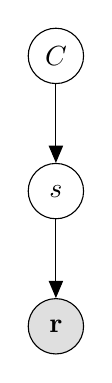
\begin{tikzpicture}
\node[obs]                               (r) {$\mathbf{r}$};
  \node[latent, above=of r] (s) {$s$};
   \node[latent, above=of s]  (c) {$C$};
   \edge {c} {s};
  \edge {s} {r}; 
 \end{tikzpicture}
 \\
$C$ is the category distribution ($\in \{0, 1\})$\\
$P(C) = .5$\\ 
$s$ is the presented stimulus, a draw from the selected category distribution\\
$P(s|C) = \mathcal{N} (s; 0, \sigma_{\text{C}}^2) = \mathcal{N} (s; 0, \tau_{\text{C}}^{-1})$\\
$\mathbf{r}$ is the vector of neural responses to $s$:
$P(r_i|s) = \text{Poisson}(r_i; f_i(s))$\\
~\\
$f_i(s)$ is the tuning curve of the $i^\text{th}$ neuron in response to a stimulus $s$\\
Tuning curve assumptions:
\begin{itemize}
\item Tuning curves cover the space so $\sum_i f_i(s)$ is independent of $s$
\item The tuning curves are Gaussian: $f_i(s) \sim \mathcal{N} (s_i^{\text{pref}}, \sigma_{\text{tc}}^2)$
\end{itemize}

\subsection{Inference}
\begin{equation}
\begin{aligned}
P(C, s|\mathbf{r}) &= \Big(\prod_i P(r_i|s)\Big) P(s|C) P(C)\\
&\propto \Big(\prod_i \text{Poisson}(r_i; f_i(s))\Big) \mathcal{N} (s; 0, \tau_{\text{C}}^{-1})\\
&= \Big(\prod_i \frac{f_i(s)^{r_i}}{r_i!} \Big) \sqrt{\frac{\tau_C}{2 \pi}} e^{\frac{-\tau_C s^2}{2}}
\end{aligned}
\end{equation}

Let 
\begin{equation}
\begin{aligned}
\tau_C &= \begin{cases}
\tau_0, & \text{if } C = 0\\
\tau_1, & \text{if } C = 1
\end{cases}\\
&= \tau_0 (1 - C) + \tau_1 C\\
&= \tau_0 - (\tau_0 - \tau_1)C\\
&= \tau_0 - C \Delta \tau
\end{aligned}
\end{equation}

For variational inference,
\begin{equation}
\begin{aligned}
\log P(C, s|\mathbf{r}) &= \sum_i \Big(- \log r_i! + r_i \log(f_i(s)) \Big) + \frac{-(\tau_0 - C \Delta \tau) s^2}{2} + \frac{1}{2} \log \Big(\frac{\tau_0 - C \Delta \tau}{2 \pi} \Big)
\end{aligned}
\end{equation}

\subsection{Variational approximation}
Then we approximate this using a factorized distribution:
\begin{equation}
Q(C, s|\mathbf{r}) = Q(C|\mathbf{r}) Q(s|\mathbf{r})
\end{equation}

\begin{equation}
\begin{aligned}
\log Q(C|\mathbf{r}) &= \langle \log P(C, s|\mathbf{r}) \rangle_{Q(s|\mathbf{r})}\\
&= \frac{C \Delta \tau}{2} \langle s^2 \rangle_{Q(s|\mathbf{r})} + \frac{1}{2} \log \Big(\frac{\tau_0 - C \Delta \tau}{2 \pi} \Big)\\
&\propto \frac{C \Delta \tau}{2} \langle s^2 \rangle_{Q(s|\mathbf{r})} + \frac{1}{2} \log (\tau_0 - C \Delta \tau)\\
\log Q(C = 1|\mathbf{r}) &\propto \frac{\Delta \tau}{2} \langle s^2 \rangle_{Q(s|\mathbf{r})} + \frac{1}{2} \log (\tau_0 - \Delta \tau)\\
\log Q(C = 0|\mathbf{r}) &\propto \frac{1}{2} \log (\tau_0)\\
\log \frac{Q(C = 1|\mathbf{r})}{Q(C = 0|\mathbf{r})} &= \frac{\Delta \tau}{2} \langle s^2 \rangle_{Q(s|\mathbf{r})} + \frac{1}{2} \log \Big( \frac{\tau_1}{\tau_0} \Big)\\
Q(C = 1|\mathbf{r}) &= \frac{1}{1 + e^{-\log \frac{Q(C = 1|\mathbf{r})}{Q(C = 0|\mathbf{r})}}}\\
Q(C|\mathbf{r}) & \sim \text{Bernoulli}(p)\\
p &= \frac{1}{1 + \sqrt{\frac{\tau_0}{\tau_1}} e^{- \frac{\Delta \tau}{2} \langle s^2 \rangle_{Q(s|\mathbf{r})}}}
\end{aligned}
\end{equation}

\begin{equation}
\begin{aligned}
Q(s|\mathbf{r}) &= \langle \log P(C, s|\mathbf{r}) \rangle_{Q(C|\mathbf{r})}\\
&= \sum_i r_i \log(f_i(s)) + \frac{- (\tau_0 - \langle C \rangle_{Q(C|\mathbf{r})} \Delta \tau)}{2} s^2\\
&\propto \frac{1}{2 \sigma^2_{\text{tc}}} \sum_i r_i (s - s_i^{\text{pref}})^2 + \frac{- (\tau_0 - \langle C \rangle_{Q(C|\mathbf{r})} \Delta \tau)}{2} s^2\\
&\sim \mathcal{N} (\mu, \tau)\\
\tau &= \sum_i \frac{r_i}{\sigma^2_{\text{tc}}}+ (\tau_0 - \langle C \rangle_{Q(C|\mathbf{r})} \Delta \tau)\\
&= \sum_i \frac{r_i}{\sigma^2_{\text{tc}}}+ (\tau_0 - p \Delta \tau)\\
\mu &= \frac{\sum_i \frac{r_i}{\sigma^2_{\text{tc}}}s_i^{\text{pref}}}{\sum_i \frac{r_i}{\sigma^2_{\text{tc}}}+ (\tau_0 - \langle C \rangle_{Q(C|\mathbf{r})} \Delta \tau)}\\
&= \frac{\sum_i \frac{r_i}{\sigma^2_{\text{tc}}}s_i^{\text{pref}}}{\tau}\\
\eta &= \mu \tau\\
&= \sum_i \frac{r_i}{\sigma^2_{\text{tc}}}s_i^{\text{pref}}
\end{aligned}
\end{equation}

($\eta$ and $\tau$ are natural parameters)

Also

\begin{equation}
\begin{aligned}
\langle s^2 \rangle_{Q(s|\mathbf{r})} &= (\frac{\eta}{\tau})^2 + \frac{1}{\tau}\\
\end{aligned}
\end{equation}

So we have update equations ($\eta$ is a constant):
\begin{equation}
\begin{aligned}
\frac{dp}{dt} &= 1 - p(1 + \sqrt{\frac{\tau_0}{\tau_1}} e^{-\frac{((\frac{\eta}{\tau})^2 + \frac{1}{\tau}) \Delta \tau}{2}})\\
\frac{d \tau}{dt} &= -\tau + \sum_i \frac{r_i}{\sigma^2_{\text{tc}}}+ (\tau_0 - p \Delta \tau)\\
\end{aligned}
\end{equation}

Analytic posterior:

From Qamar et al. (2013) we have
\begin{equation}
\begin{aligned}
\sigma_0^2 &= \frac{1}{\tau_0}\\
\sigma_1^2 &= \frac{1}{\tau_1}\\
\log \frac{P(\mathbf{r}|C = 0)}{P(\mathbf{r}|C = 1)} &= \frac{1}{2} \log \frac{1 + \sigma_1^2 \mathbf{a} \cdot \mathbf{r}}{1 + \sigma_0^2\mathbf{a} \cdot \mathbf{r}} - \frac{(\sigma_1^2 - \sigma_0^2)(\mathbf{b} \cdot \mathbf{r})^2}{2 (1 + \sigma_0^2 \mathbf{a} \cdot \mathbf{r})(1 + \sigma_1^2 \mathbf{a} \cdot \mathbf{r})}\\
P(\mathbf{r}|C = 0) &= \frac{1}{1 + e^{-(\frac{1}{2} \log \frac{1 + \sigma_1^2 \mathbf{a} \cdot \mathbf{r}}{1 + \sigma_0^2\mathbf{a} \cdot \mathbf{r}} - \frac{(\sigma_1^2 - \sigma_0^2)(\mathbf{b} \cdot \mathbf{r})^2}{2 (1 + \sigma_0^2 \mathbf{a} \cdot \mathbf{r})(1 + \sigma_1^2 \mathbf{a} \cdot \mathbf{r})})}}
\end{aligned}
\end{equation}

\end{document}